\chapter{implémentations mise en service et test}
\fancyhead[R]{\textit{implémentations mise en service et test}}
\renewcommand{\headrulewidth}{1pt}

\section{Introduction}
Ce chapitre sera d'abord consacré à la présentation de l’environnent de
développement et des librairies utilisées. Ensuite, nous expliquerons
l’architecture globale du système ainsi que son principe de fonctionnement. La
deuxième partie sera réservée à la présentation de l’application dans ses
différents aspects en commençant par sa charte graphique et la hiérarchie des
pages de l’application web. Enfin, nous illustrerons quelques interfaces issues
de l’application et nous aborderons brièvement le côté sécurité de l’application
réalisée.   

\section{Environnement de développement}
Un environnement de développement se réfère à une suite d’applications et 
d’outils qui permettent un développement d’application facile. Par exemple, 
gérer des fichiers sources, déboguer du code, et enfin tester l’application 
avant de la lancer sur un environnement de test ou de production. Dans cette 
section nous allons présenter l’environnement de développement utilisé pour 
développer notre application web.

\subsection{Plateformes utilisés}

\subsubsection*{Slack}
\begin{wrapfigure}{r}{0.09\textwidth}
    \vspace{-22pt}
    \begin{center}
        
\includegraphics[scale=0.36]{images/logo/slack.png}
        \label{fig62}
    \end{center}
    \vspace{-20pt}
    \vspace{-10pt}
\end{wrapfigure}

Slack est une plateforme de communication collaborative propriétaire, elle 
permet de faciliter l’organisation grâce à un système de canaux centralisant 
tout ce qui concerne un projet, un sujet ou une équipe. Elle permet également 
de conserver les fichiers et les messages partager dans ces canaux\cite{37}. 

\clearpage

\subsubsection*{Trello}
\begin{wrapfigure}{r}{0.09\textwidth}
    \vspace{-22pt}
    \begin{center}
        
\includegraphics[scale=0.36]{images/logo/trello.png}
        \label{fig63}
    \end{center}
    \vspace{-20pt}
    \vspace{-10pt}
\end{wrapfigure}

Trello est un outil de gestion de projet en ligne, lancé en septembre 2011. Il 
repose sur une organisation des projets en planches listant des cartes, chacune 
représentant des tâches. Les cartes sont assignables à des utilisateurs et sont 
mobiles d’une planche à l’autre, traduisant leur avancement. Il permet donc 
d’organiser les projets et de définir leur ordre de priorité de façon amusante, 
souple et enrichissante\cite{38}.

\subsubsection*{Github}
\begin{wrapfigure}{r}{0.09\textwidth}
    \vspace{-22pt}
    \begin{center}
        
\includegraphics[scale=0.36]{images/logo/github.png}
        \label{fig64}
    \end{center}
    \vspace{-20pt}
    \vspace{-10pt}
\end{wrapfigure}

GitHub est une plateforme de développement qui offre un service d’hébergement 
qui permet aux développeurs de stocker et de partager, publiquement ou non, 
le code qu’ils créent. Elle fournit aussi plusieurs fonctionnalités de 
collaboration, telles que des wikis et des outils de gestion des tâches de base 
pour chaque projet\cite{40}.

\subsubsection*{Discord}
\begin{wrapfigure}{r}{0.09\textwidth}
    \vspace{-22pt}
    \begin{center}
        
\includegraphics[scale=0.36]{images/logo/discord.png}
        \label{fig65}
    \end{center}
    \vspace{-20pt}
    \vspace{-10pt}
\end{wrapfigure}

Discord est une plateforme gratuite qui offre un service de communication par 
chat vidéo, vocal et textuel, il est donc utile et nécessaire de l’utiliser pour 
une communication en continu surtout en temps de pandémie\cite{40}.

\subsection{Logiciels utilisés}
\subsubsection*{Visual studio code}
\begin{wrapfigure}{r}{0.09\textwidth}
    \vspace{-20pt}
    \begin{center}
        
\includegraphics[width=0.09\textwidth]{images/VSCode logo.png}
        \label{fig66}
    \end{center}
    \vspace{-20pt}
    \vspace{-10pt}
\end{wrapfigure}

Visual Studio Code (VSCode) est un éditeur de code source, développé par 
Microsoft en tant que projet open source. Il s’agit de l’outil d’environnement 
de développement le plus populaire au monde selon un sondage auprès des 
développeurs réalisé par Stackoverflow\cite{13}. En plus d’être un éditeur open 
source, il dispose d’un contrôle de gestion intégrée et d’un grand nombre 
d’extensions\cite{41}.

\subsubsection*{Git}
\begin{wrapfigure}{r}{0.09\textwidth}
    \vspace{-28pt}
    \begin{center}
        
\includegraphics[width=0.09\textwidth]{images/git logo.png}
        \label{fig67}
    \end{center}
    \vspace{-20pt}
    \vspace{-10pt}
\end{wrapfigure}   

Git est un logiciel de gestion de versions décentralisé. C’est un logiciel libre 
créé par Linus Torvalds, auteur du noyau Linux en 2016. Il s’agit du logiciel 
de gestion de versions le plus populaire qui est utilisé par plus de douze 
millions de personnes\cite{43}.

\subsubsection*{Conda}
\begin{wrapfigure}{r}{0.09\textwidth}
    \vspace{-36pt}
    \begin{center}
        
\includegraphics[width=0.09\textwidth]{images/Conda logo.png}
        \label{fig68}
    \end{center}
    \vspace{-20pt}
    \vspace{-10pt}
\end{wrapfigure}

Conda est un système de gestion de paquets open source et un système de gestion
d’environnement qui permet d’installer, exécuter et de mettre à jour rapidement
les packages et leurs dépendances ainsi que l’installation de multiples versions
de logiciels au travers d’un mécanisme d’environnements virtuels\cite{44}.

\subsubsection*{Adobe XD}
\begin{wrapfigure}{r}{0.09\textwidth}
    \vspace{-22pt}
    \begin{center}
        
\includegraphics[scale=0.36]{images/logo/adobexd.png}
        \label{fig69}
    \end{center}
    \vspace{-20pt}
    \vspace{-10pt}
\end{wrapfigure}

C’est une solution d’UX/UI design complète pour la conception de sites web, 
d’applications mobiles, etc.

C’est un outil performant pour créer des flux utilisateur, des wireframes, des
maquettes extrêmement fidèles, des prototypes interactifs, des animations. Il
permet aussi de modifier et de partager facilement des prototypes interactifs
avec des collaborateurs sur l’ensemble des appareils et des
plates-formes\cite{45}.

\subsection{technologie utilisée}
Dans cette section, nous allons présenter les différentes technologies utilisé
pour développer notre application web.

\subsection{HTML}
\begin{wrapfigure}{r}{0.09\textwidth}
    \vspace{-22pt}
    \begin{center}
        
\includegraphics[scale=0.36]{images/logo/html.png}
        \label{fig70}
    \end{center}
    \vspace{-20pt}
    \vspace{-10pt}
\end{wrapfigure}

C'est un langage de balisage principal du World Wide Web. À l'origine, HTML 
était principalement conçu comme un langage pour décrire sémantiquement des 
documents scientifiques. Sa conception générale lui a toutefois permis de 
s’adapter, au cours des années suivantes, pour décrire un certain nombre 
d’autres types de documents et même d’applications\cite{14}.

\subsection{CSS}
\begin{wrapfigure}{r}{0.09\textwidth}
    \vspace{-22pt}
    \begin{center}
        
\includegraphics[scale=0.36]{images/logo/css.png}
        \label{fig71}
    \end{center}
    \vspace{-20pt}
    \vspace{-10pt}
\end{wrapfigure}

Les feuilles de style en cascade sont un mécanisme simple pour ajouter du style 
(par exemple, polices, couleurs, espacement) aux documents Web. Les standards le 
définissant sont publiés par le World Wide Web Consortium (W3C)\cite{15}.

\subsection{Sass}
\begin{wrapfigure}{r}{0.09\textwidth}
    \vspace{-22pt}
    \begin{center}
        
\includegraphics[scale=0.36]{images/logo/sass.png}
        \label{fig72}
    \end{center}
    \vspace{-20pt}
    \vspace{-10pt}
\end{wrapfigure}

Sass est un langage de feuille de style compilé en CSS. Il permet d'utiliser des 
variables, des règles imbriquées, des mixins, des fonctions, etc., Le tout 
avec une syntaxe entièrement compatible CSS. Il permet aussi de garder les 
feuilles de style bien organisées et facilite le partage de la conception au 
sein et entre les projets\cite{46}.

\clearpage        

\subsection{JavaScript}
\begin{wrapfigure}{r}{0.09\textwidth}
    \vspace{-22pt}
    \begin{center}
        
\includegraphics[scale=0.36]{images/logo/js.png}
        \label{fig73}
    \end{center}
    \vspace{-20pt}
    \vspace{-10pt}
\end{wrapfigure}

JavaScript est un langage de programmation de scripts principalement employé 
dans les pages web interactives et à ce titre est une partie essentielle des 
applications web. Avec les technologies HTML et CSS, JavaScript est parfois 
considéré comme l'une des technologies cœur du World Wide Web\cite{16}.     

\subsection{Python}
\begin{wrapfigure}{r}{0.09\textwidth}
    \vspace{-22pt}
    \begin{center}
        
\includegraphics[scale=0.36]{images/logo/python.png}
        \label{fig74}
    \end{center}
    \vspace{-20pt}
    \vspace{-10pt}
\end{wrapfigure}

Python est un langage de programmation puissant et facile à apprendre. Il a des 
structures de données de haut niveau efficaces et une approche simple, mais 
efficace de la programmation orientée objet. La syntaxe élégante et le typage 
dynamique de Python, ainsi que sa nature interprétée, en font un langage idéal 
pour la création de scripts et le développement rapide d’applications dans de 
nombreux domaines sur la plupart des plates-formes\cite{17}.

\subsection{Django}
\begin{wrapfigure}{r}{0.12\textwidth}
    \vspace{-22pt}
    \begin{center}
        
\includegraphics[scale=0.5]{images/logo/django.png}
        \label{fig75}
    \end{center}
    \vspace{-20pt}
    \vspace{-10pt}
\end{wrapfigure}

Django est un framework Web Python de haut niveau open source qui encourage un
développement rapide et une conception propre et pragmatique. Conçu par des
développeurs expérimentés, il prend en charge une grande partie des tracas du
développement Web. Il permet l'écriture des applications web sans avoir à
réinventer la roue\cite{18}.

Il est basé sur l' architecture MVT, qui est un modèle de conception de logiciel 
composé des 3 parties suivantes:

\begin{description}
    \item[Model:] Un modèle est la source d’information unique et définitive à
        propos des données. Il contient les champs et le comportement essentiels
        des données stockées. Généralement, chaque modèle correspond à une seule
        table de base de données\cite{19}.
    \item[View:] Une vue, pour faire simple, est une fonction Python acceptant
        une requête Web et renvoyant une réponse Web. Cette réponse peut
        contenir le contenu HTML d’une page Web, une redirection, une erreur
        404, un document XML, une image… ou vraiment n’importe quoi d’autre. La
        vue elle-même contient la logique nécessaire pour renvoyer une
        réponse\cite{20}.
    \item[Template:] Par sa nature liée au Web, Django a besoin d’un procédé
        agile de génération dynamique de HTML. L’approche la plus couramment
        utilisée est de se baser sur des templates. Un template contient la
        partie statique du résultat HTML souhaité ainsi qu’une certaine syntaxe
        particulière définissant comment insérer le contenu dynamique\cite{21}.
\end{description}

\section{Persistance des données}
Pour les données, Django comprend une couche ORM par défaut qui peut être 
utilisée pour interagir avec les données d'application de diverses bases de 
données relationnelles telles que SQLite, PostgreSQL et MySQL.

\subsection{MySql}
\begin{wrapfigure}{r}{0.14\textwidth}
    \vspace{-22pt}
    \begin{center}
        
\includegraphics[scale=0.36]{images/logo/mysql.png}
        \label{fig76}
    \end{center}
    \vspace{-20pt}
    \vspace{-10pt}
\end{wrapfigure}

MySQL est un système de gestion de bases de données relationnelles SQL open 
source développé et supporté par Oracle. Son approche relationnelle permet 
d'organiser les données dans des tableaux à deux dimensions appelés des 
relations ou tables\cite{47}.

\subsection{ORM}
Django ORM est l'un des principaux piliers de Django. Il offre une couche
d'abstraction qui permet de travailler avec des bases de données, de manière
indépendante. Il combine la facilité d'utilisation en offrant une puissante API
qui permet les opérations de base pour la persistance des données: créer,
récupérer, mettre à jour, et supprimer facilement des objets. Ainsi, il garde
les choses simples faciles et les choses difficiles possibles en offrant la
possibilité d’exécuter des requêtes SQL brutes\cite{48}.

\begin{figure}[h!]
    \centering
    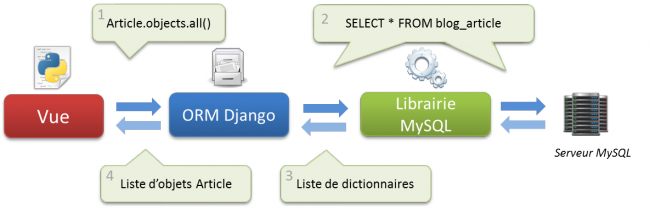
\includegraphics[scale=0.8 ]{images/ORM.png}
    \label{fig77}
    \caption{Fonctionnement de l'ORM de Django}
    \label{}
\end{figure}

\clearpage       

\section{Les librairies utilisées}
\subsection{Bootstrap}
\begin{wrapfigure}{r}{0.09\textwidth}
    \vspace{-22pt}
    \begin{center}
        
\includegraphics[scale=0.36]{images/logo/bootstrap.png}
        \label{fig78}
    \end{center}
    \vspace{-20pt}
    \vspace{-10pt}
\end{wrapfigure}

C’est le framework css le plus populaire au monde pour créer des sites 
responsifs et adaptés aux mobiles. Il dispose d’un système de grille réactif, 
de nombreux composants prédéfinis et de puissants plugins JavaScript\cite{22}.

\subsection{JQuery}
\begin{wrapfigure}{r}{0.09\textwidth}
    \vspace{-22pt}
    \begin{center}
        
\includegraphics[scale=0.36]{images/logo/jquery.png}
        \label{fig79}
    \end{center}
    \vspace{-20pt}
    \vspace{-10pt}
\end{wrapfigure}

jQuery est une bibliothèque JavaScript rapide, petite, et riche en
fonctionnalités. Il simplifie considérablement le parcours et la manipulation de
documents HTML, la gestion des événements, l'animation grâce à une API facile à
utiliser qui fonctionne sur une multitude de navigateurs\cite{23}.

\subsection{Crispy forms}
Django crispy-form permet de construire, personnaliser et réutiliser des
formulaires en utilisant du css. Il permet d'éviter d'écrire beaucoup de code
dans les templates et applique la philosophie DRY\cite{24}.

\subsection{Pillow}
\begin{wrapfigure}{r}{0.09\textwidth}
    \vspace{-22pt}
    \begin{center}
        
\includegraphics[scale=0.36]{images/logo/pillow.png}
        \label{fig80}
    \end{center}
    \vspace{-20pt}
    \vspace{-10pt}
\end{wrapfigure}

C’est une bibliothèque de traitement d'images pour le langage de programmation
Python. Elle permet d'ouvrir, de manipuler, et de sauvegarder différents formats 
de fichiers graphiques\cite{25}.

\subsection{Django import/export}
django-import-export est une application et une bibliothèque Django pour
l'importation et l'exportation de données avec l'intégration d'administration
incluse\cite{26}.

\subsection{Popper}
\begin{wrapfigure}{r}{0.09\textwidth}
    \vspace{-22pt}
    \begin{center}
        
\includegraphics[scale=0.36]{images/logo/popper.png}
        \label{fig81}
    \end{center}
    \vspace{-20pt}
    \vspace{-10pt}
\end{wrapfigure}

Popper facilite le positionnement des infobulles et des popovers, il
positionnera tout élément d'interface utilisateur qui sort du flux d’un document
et flotte près d'un élément cible. L'exemple le plus courant est une infobulle.
Mais elle comprend également des popovers, des listes déroulantes, etc. Tous ces
éléments peuvent être décrits de manière générique comme un élément
popper\cite{27}.

\subsection{Font Awesome}
\begin{wrapfigure}{r}{0.09\textwidth}
    \vspace{-22pt}
    \begin{center}
        
\includegraphics[scale=0.36]{images/logo/fontawesome.png}
        \label{fig82}
    \end{center}
    \vspace{-20pt}
    \vspace{-10pt}
\end{wrapfigure}

C’est la librairie d'icônes la plus populaire d'Internet, elle facilite
l’utilisation  d’icônes de différentes variantes (Solid, Regular, Light et
Brand) en utilisant un préfixe de style et le nom de l'icône\cite{28}.

\subsection{Chart.js}
\begin{wrapfigure}{r}{0.09\textwidth}
    \vspace{-22pt}
    \begin{center}
        
\includegraphics[scale=0.36]{images/logo/chartjs.png}
        \label{fig83}
    \end{center}
    \vspace{-20pt}
    \vspace{-10pt}
\end{wrapfigure}

Chart.js est une bibliothèque JavaScript open-source gratuite créée par le 
développeur Web londonien Nick Downie en 2013. Elle est maintenant maintenue par 
la communauté, et permet la visualisation de données sur plusieurs types de 
graphiques tout en étant facile et flexible\cite{29}.

\section{Architecture du système} 
La figure présente l’architecture de notre système qui est composé en deux
parties. la première partie permet d’interagir directement avec la pointeuse
biométrique qui va consommer l’api RESTful fournie par notre application Django
qui est accessible à travers les endpoint suivants:

\begin{longtable}{|p{2.5cm}|p{4.5cm}|p{4.5cm}|p{4.5cm}|}
    % header and footer information
    \endhead
    \endfoot
    % body of table
    \hline
    Resource & GET & POST & DELETE \\
    \hline
    pointage/bio & Récupère l'identifiant d'une empreinte. & Envoi l'identifiant
    d'une empreinte. & Supprime une empreinte.
    \\
    \hline
    \caption{Endpoint de l'api RESTful}\\
\end{longtable}

La deuxième partie c’est l’application web est accessible via un navigateur
web, est présentée en détail dans la section suivante.

\vspace{10pt}
\begin{figure}[h!]
    \centering
    \includegraphics[scale=0.58 ]{images/Architecture du système.png}
    \label{fig84}
    \caption{Architecture du système}
    \label{figUFE}
\end{figure} 

\clearpage        
\section{Présentation de l'application}

\subsection{Nom et logo de l'application}
Nous avons décidé de nommer cette application \emph{'ATime'} qu’on peut traduire
par \emph{à temps} ou par \emph{au moment} pour faire référence au temps ainsi
qu’au pointage et au fait d'arriver à l'heure.

\begin{figure}[h!]
    \centering
    
\includegraphics[scale=0.4 ]{images/app_name_dark.png}
    \label{fig85}
    \caption{Nom de l'application}
    \label{}
\end{figure} 

Pour le logo, nous avons pensé à une forme qui combine une empreinte et une 
horloge deux concepts primordiaux du projet.

\begin{figure}[!htb]
    \begin{minipage}{0.5\textwidth}
        \centering
        
\includegraphics[scale=0.19]{images/applogo_bw.png}
        \caption{Logo avec couleur uniforme}\label{fig86}
    \end{minipage}\hfill
    \begin{minipage}{0.5\textwidth}
        \centering
        
\includegraphics[scale=0.19]{images/applogo_light.png}
        \caption{Logo sur fond bleu}\label{fig87}
    \end{minipage}
\end{figure}

\begin{figure}[h!]
    \centering
    
\includegraphics[scale=0.22 ]{images/applogo_dark.png}
    \caption{Logo sur fond blanc}
    \label{fig88}
\end{figure} 

\subsection{Palette de couleurs}
En raison de la nature du projet et du fait qu’il soit étroitement lié au
domaine de l'entreprise, nous avons choisi des couleurs basiques et pas beaucoup
nuancées afin de ne pas provoquer un sentiment de fatigue  des yeux lors des
longues sessions d'utilisations.

\begin{figure}[h!]
    \centering
    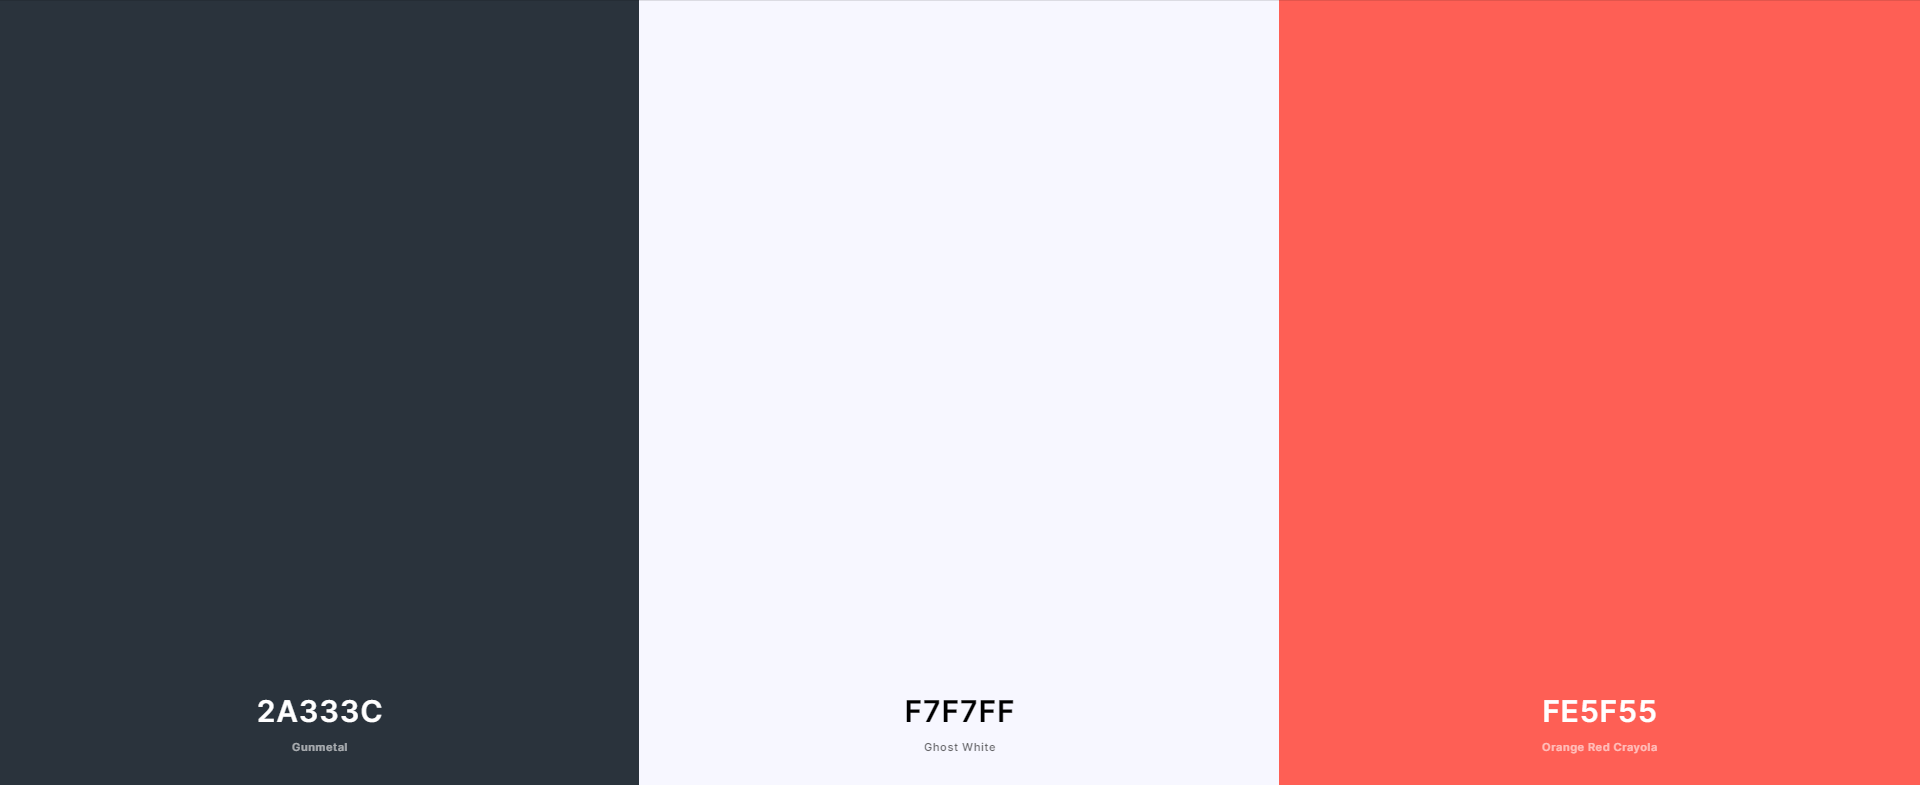
\includegraphics[scale=0.3 ]{images/palette_couleurs.PNG}
    \caption{Palette de couleur utilisé}
    \label{fig89}
\end{figure} 

\subsection{Typographie}
Le choix de la typographie de notre application repose sur le besoin d’avoir un 
rendu optimal du texte sur chaque appareil et système d'exploitation. Dans cette 
démarche, nous avons décidé de garder les polices web par défaut du framework 
bootstrap.

\subsection{Squelette de l'application web}
Le squelette d’une application web illustre la hiérarchie des différentes pages
en les distinguant par niveau de profondeur. Il permet de structurer
l’information pour que celle-ci soit claire et facilement accessible.

Dans notre application, le niveau 0 est représenté par la page 
d’authentification, les autres pages, elles aussi, sont réparties par niveaux 
en fonction du nombre de clique(s) nécessaire(s) pour se rendre dessus.

\clearpage
\thispagestyle{empty}
\begin{landscape}
    \begin{figure}[h!]
        \centering
        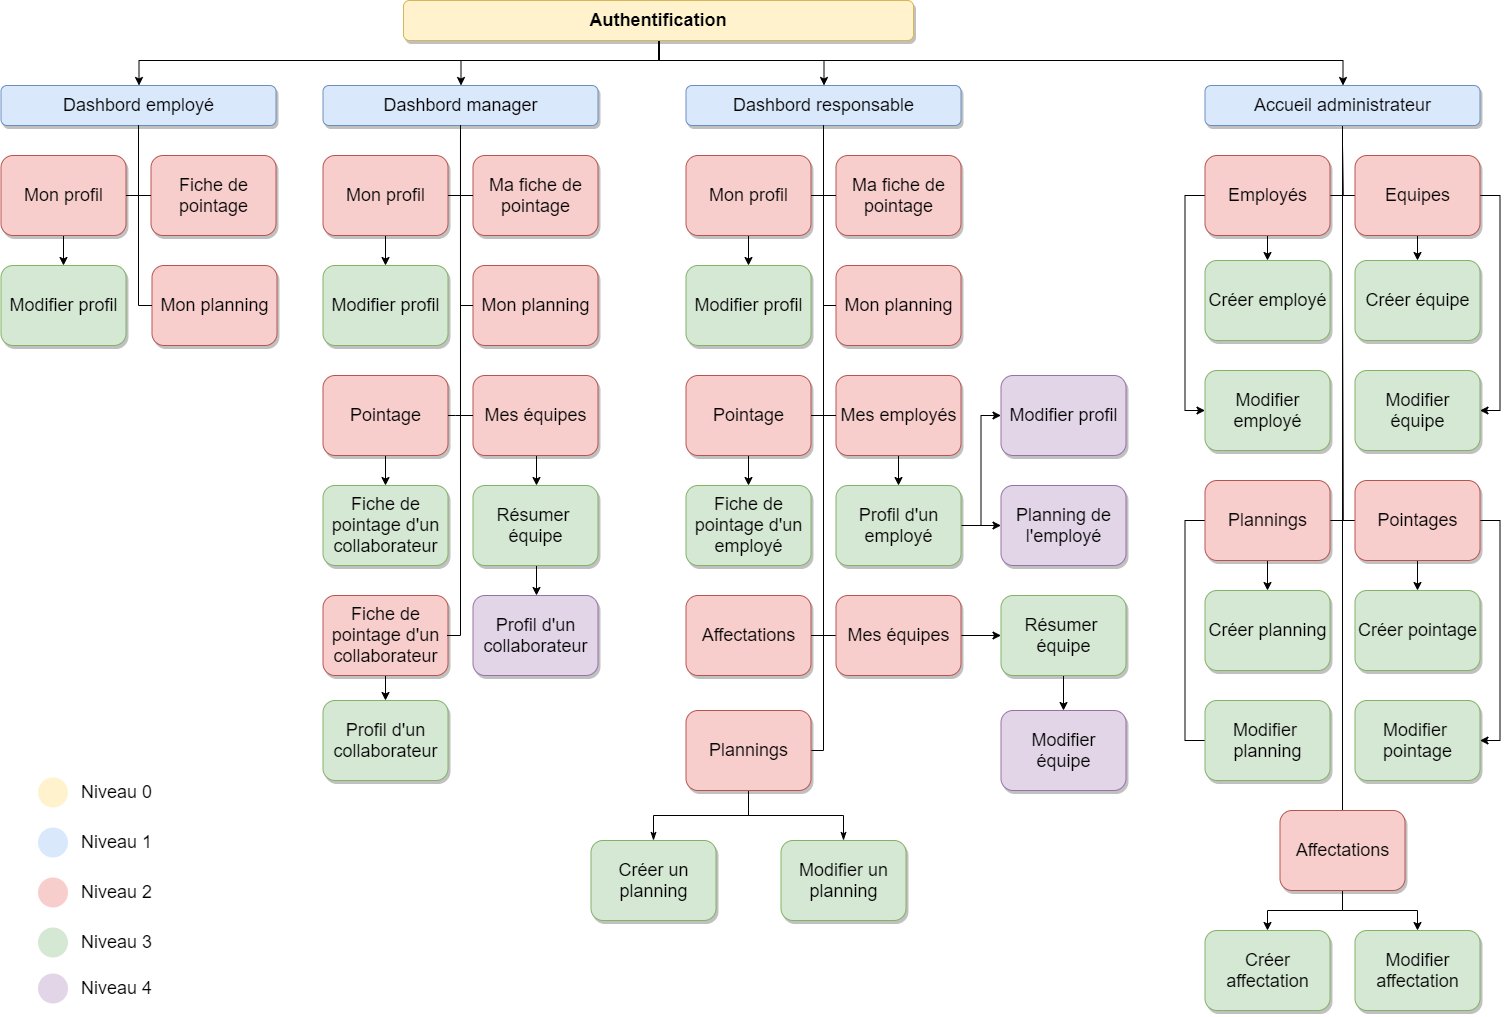
\includegraphics[scale=0.44 ]{images/interface/arbre.png}
        \caption{Squelette de l'application web}
        \label{fig90}
    \end{figure}  
\end{landscape}

\clearpage

\section{Présentation des interfaces}
Notre application comporte 4 type utilisateur, afin de présenter les principales interfaces dans
les conditions réelles d’utilisation de l’application, nous allons les présenter par espace de chaque
acteur.

\subsection{Espace employé}
En plus de l’employé cette espace est partager par plusieurs acteurs, car il comporte certains
fonctionnalités communes, ci-dessous nous avons modéliser le parcours de ce dernier à travers les
interfaces qui lui sont dédié.

\begin{figure}[h!]
    \vspace{-30pt}
    \centering
    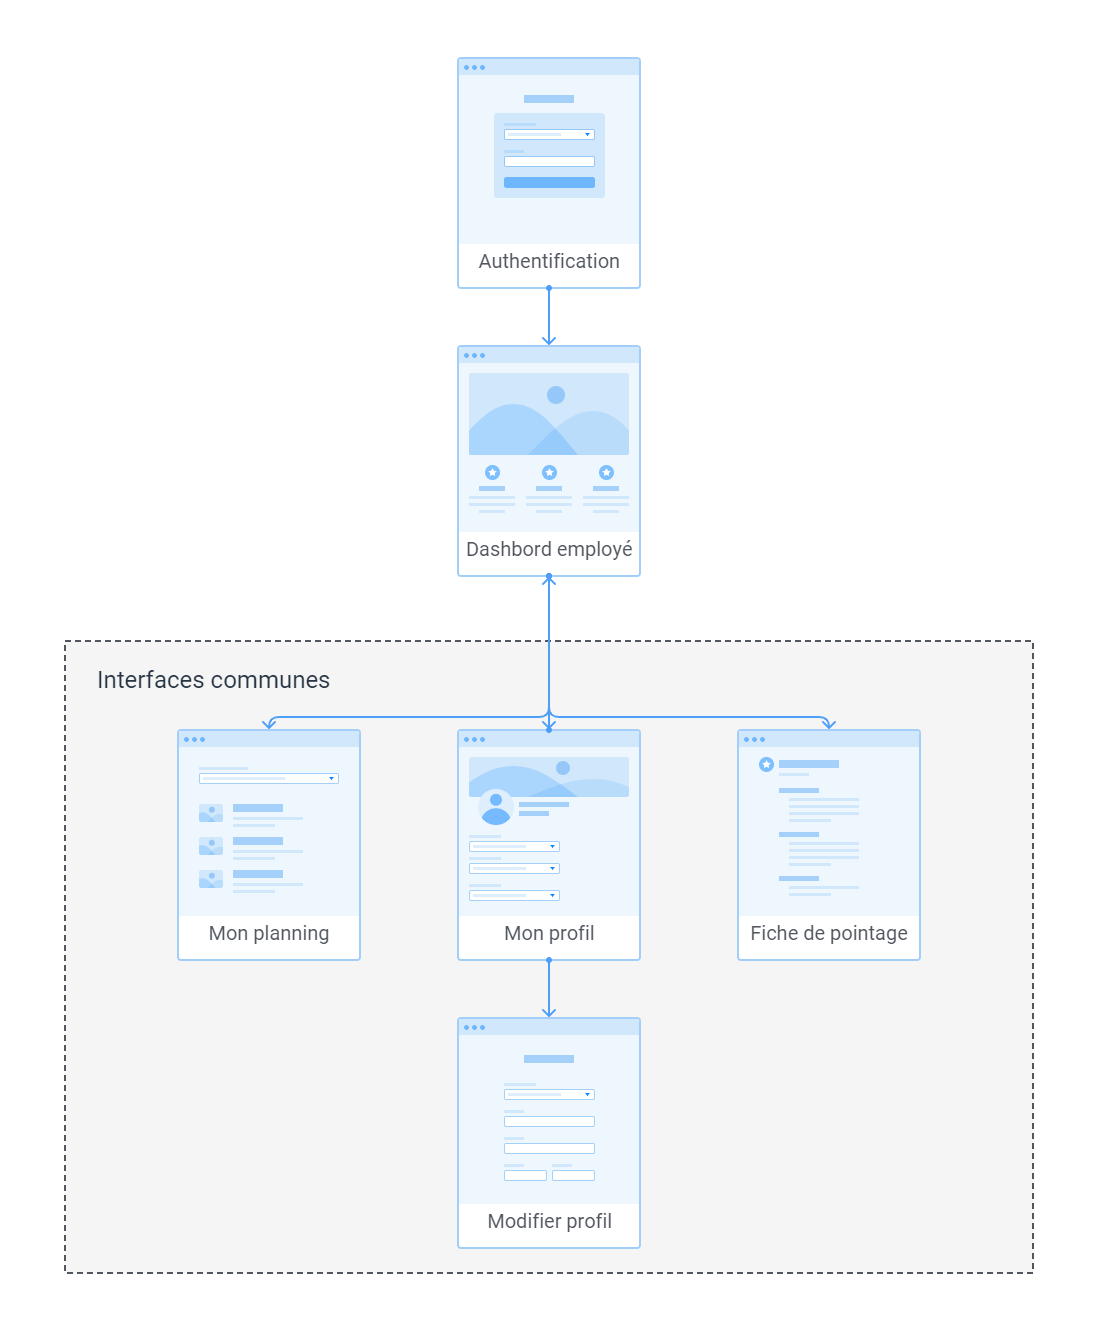
\includegraphics[scale=0.38 ]{images/interface/Espace employe.png}
    \vspace{-20pt}
    \caption{User flow de l'employé}
    \label{fig91}
\end{figure} 

\clearpage

\subsubsection*{Interface dashbord employé}
une fois que l’employé s'authentifie, il sera redirigé vers l’interface
\emph{Dashbord employé} sur laquelle il retrouve:

\begin{itemize}
    \item[\textbullet] Le nombre d’heures en poste depuis son dernier pointage.
    \item[\textbullet] Le nombre d’heures qu’il lui reste par rapport à son
        planning du jour.
    \item[\textbullet] Son planning journalier dans lequel Il a une vision
        précise de ces horaires de travails.
    \item[\textbullet] Une liste de ces collaborateurs avec les informations les
        plus utiles telle que le nom, prénom, le rôle au sein de l’entreprise,
        le genre, le numéro de téléphone professionnel et enfin un statut de
        présence/absence.
\end{itemize}

Après avoir consulté le dashbord il pourra utiliser le menu qui se trouve à 
gauche afin de naviguer à travers les différentes interfaces.

\begin{figure}[h!]
    \centering
    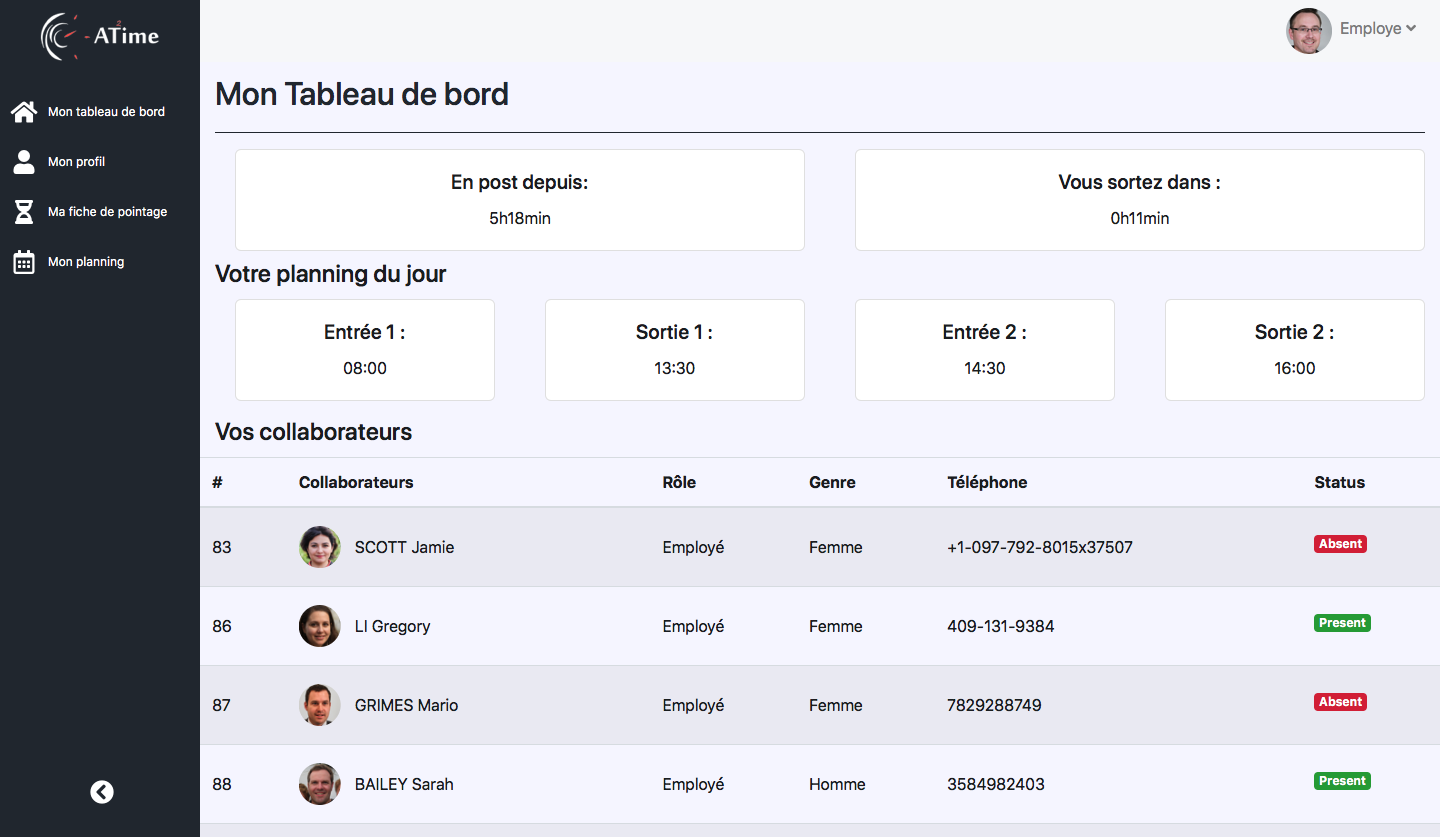
\includegraphics[scale=0.35 ]{images/interface/dashbord_employe.png}
    \caption{Interface dashbord employé}
    \label{fig92}
\end{figure}

\subsubsection*{Interface ma fiche de pointage}
Depuis cette interface, l’employé aura la possibilité de consulter la liste de 
ses pointages effectués depuis son recrutement au sein de l’entreprise et qui 
seront regroupés par date. Afin de faciliter la recherche, il aura la 
possibilité de les filtrer par semaine/mois ainsi que de faire une recherche 
précise par période.

\begin{figure}[h!]
    \vspace{-10pt}
    \centering
    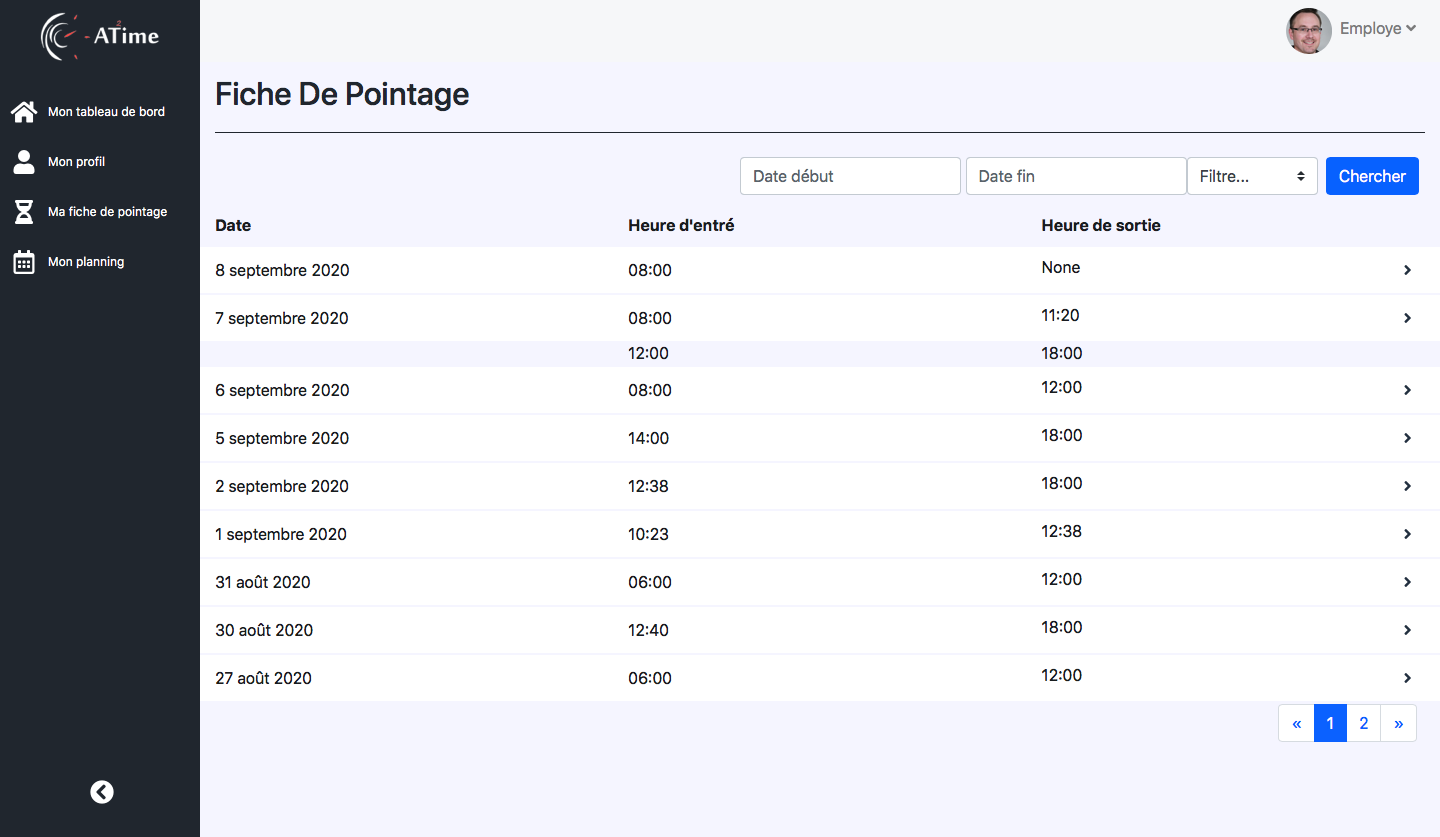
\includegraphics[scale=0.306 ]{images/interface/fiche_pointage.png}
    \caption{Interface ma fiche de pointage}
    \label{fig93}
\end{figure}

\vspace{-10pt}   
\subsubsection*{Interface consulter mon profil}
Cette interface permet à l’employé de consulter son profil qui est constitué
d’informations d'identification de base pour le bon fonctionnement du système,
ainsi que de diverses informations le concernant et qui peuvent être renseignées
par l’employé lui-même en accédant à l’interface de modification.

\begin{figure}[h!]
    \centering
    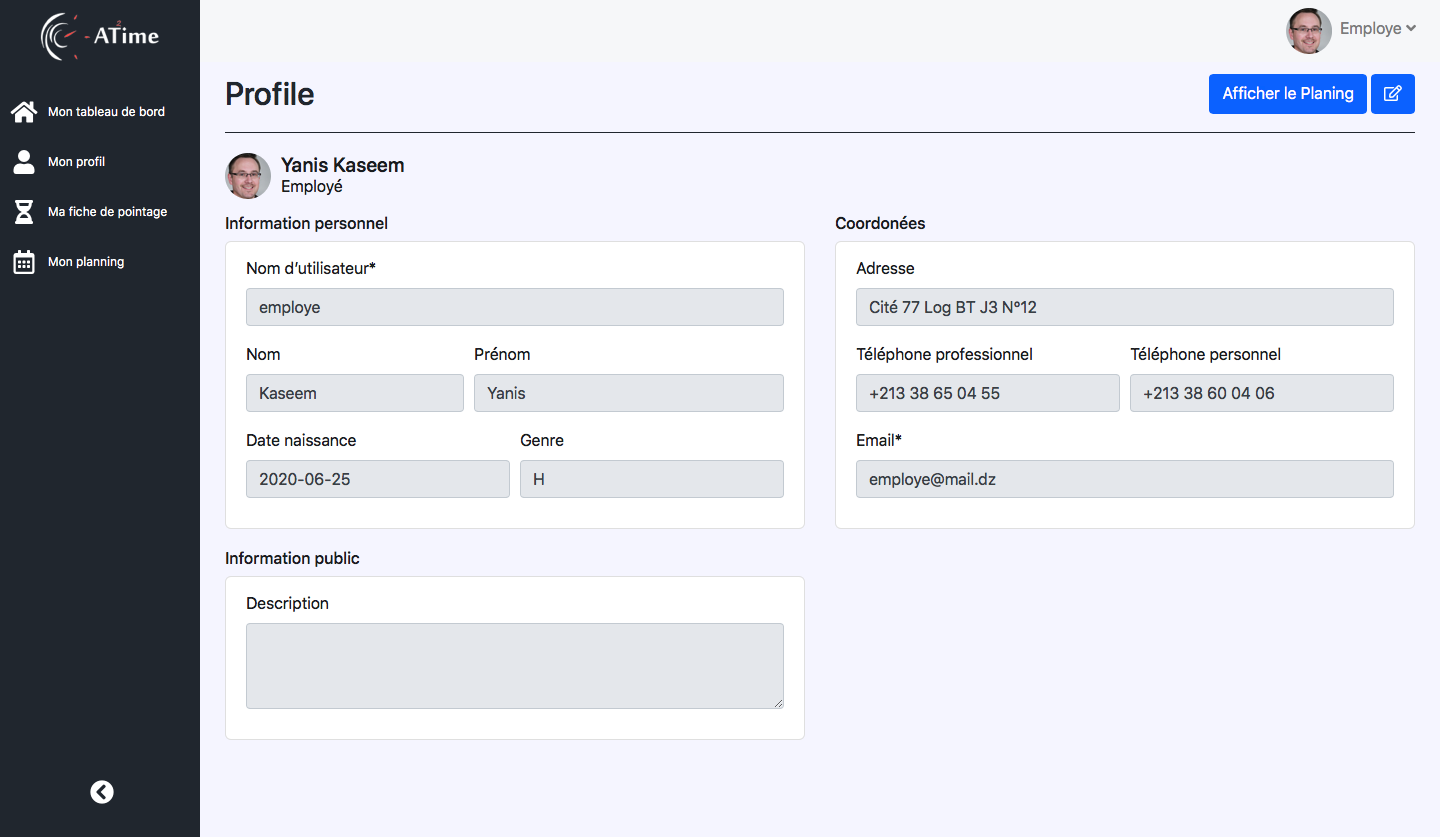
\includegraphics[scale=0.306 ]{images/interface/mon_profil.png}
    \caption{Interface consulter mon profil}
    \label{fig94}
\end{figure}

\clearpage

\subsection{Espace manager}
Cet espace qui est dédié au manager, lui permet non seulement de superviser ses
collaborateurs et ses équipes, mais aussi de profiter des fonctionnalités
partagées avec l’employé, ci-dessous nous avons modélisé le parcours du manager
à travers son espace personnel. Pour ce qui est des interfaces communes elles
sont modélisées dans la figure \ref{fig95}.

\begin{figure}[h!]
    \vspace{-10pt}
    \centering
    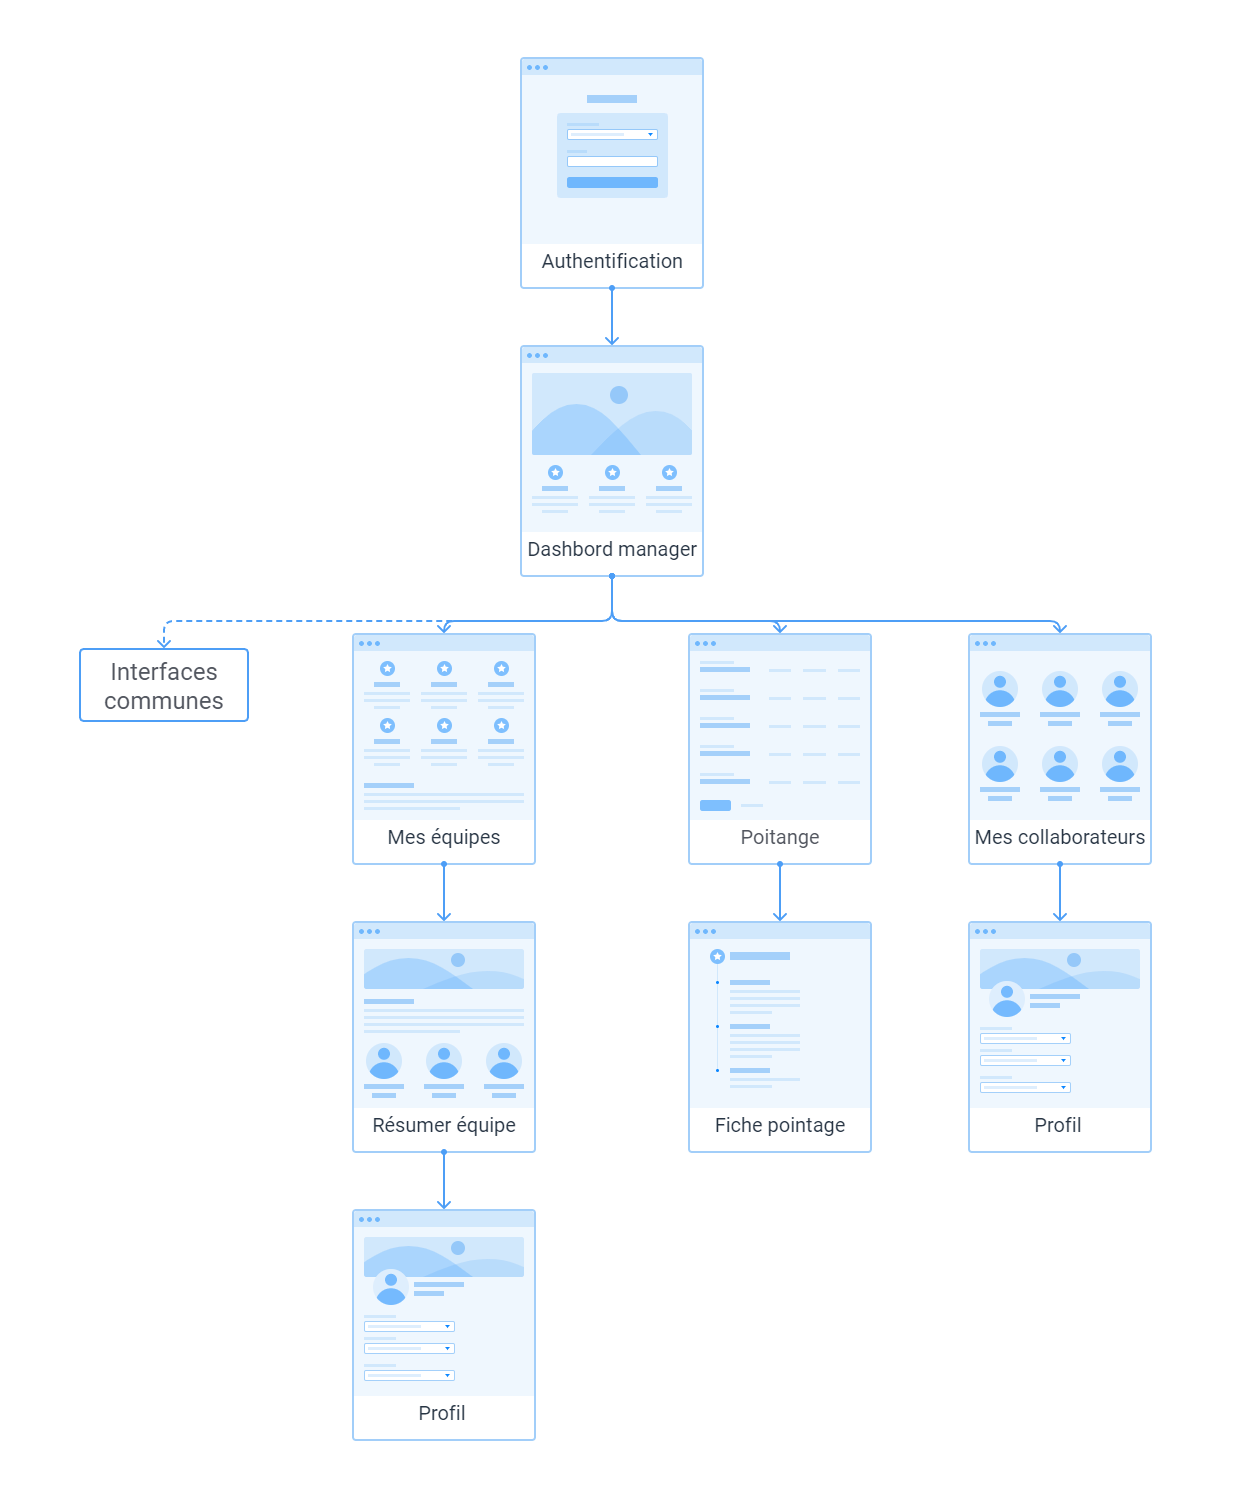
\includegraphics[scale=0.38 ]{images/interface/Espace manager.png}
    \vspace{-30pt}
    \caption{User flow du manager}
    \label{fig95}
\end{figure}

\clearpage

\subsubsection*{Interface consulter tableau de bord manager}
Une fois que le manager s'authentifie il sera redirigé vers l’interface
\emph{dashbord manager} qui contient deux onglets, le èmeer onglet est identique
à celui de l’employé, le deuxiième onglet «Mes équipes» résume les informations
des collaborateurs de ses différentes équipes. 

\begin{figure}[h!]
    \centering
    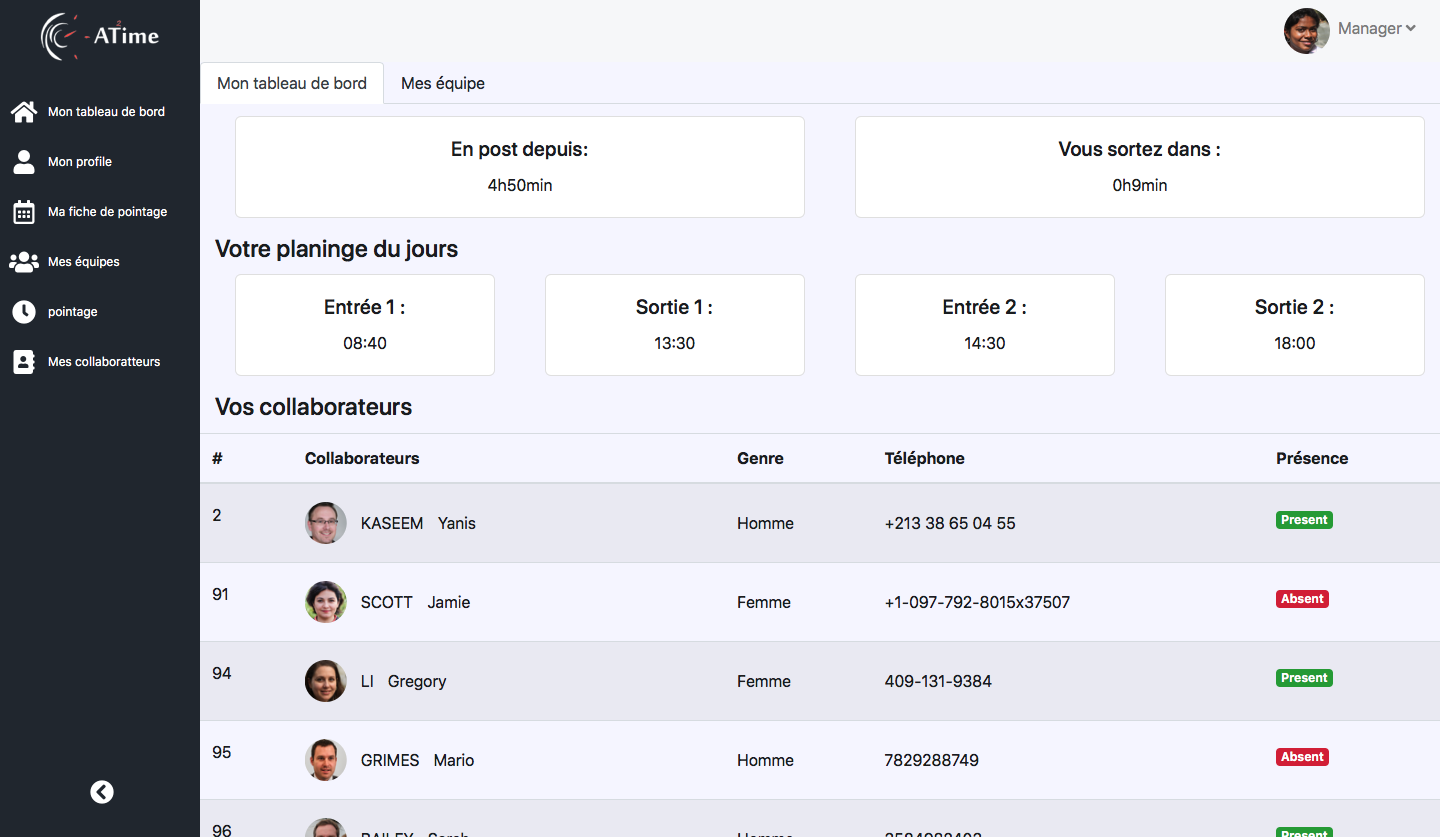
\includegraphics[scale=0.326 ]{images/interface/dashbord_manager1.png}
    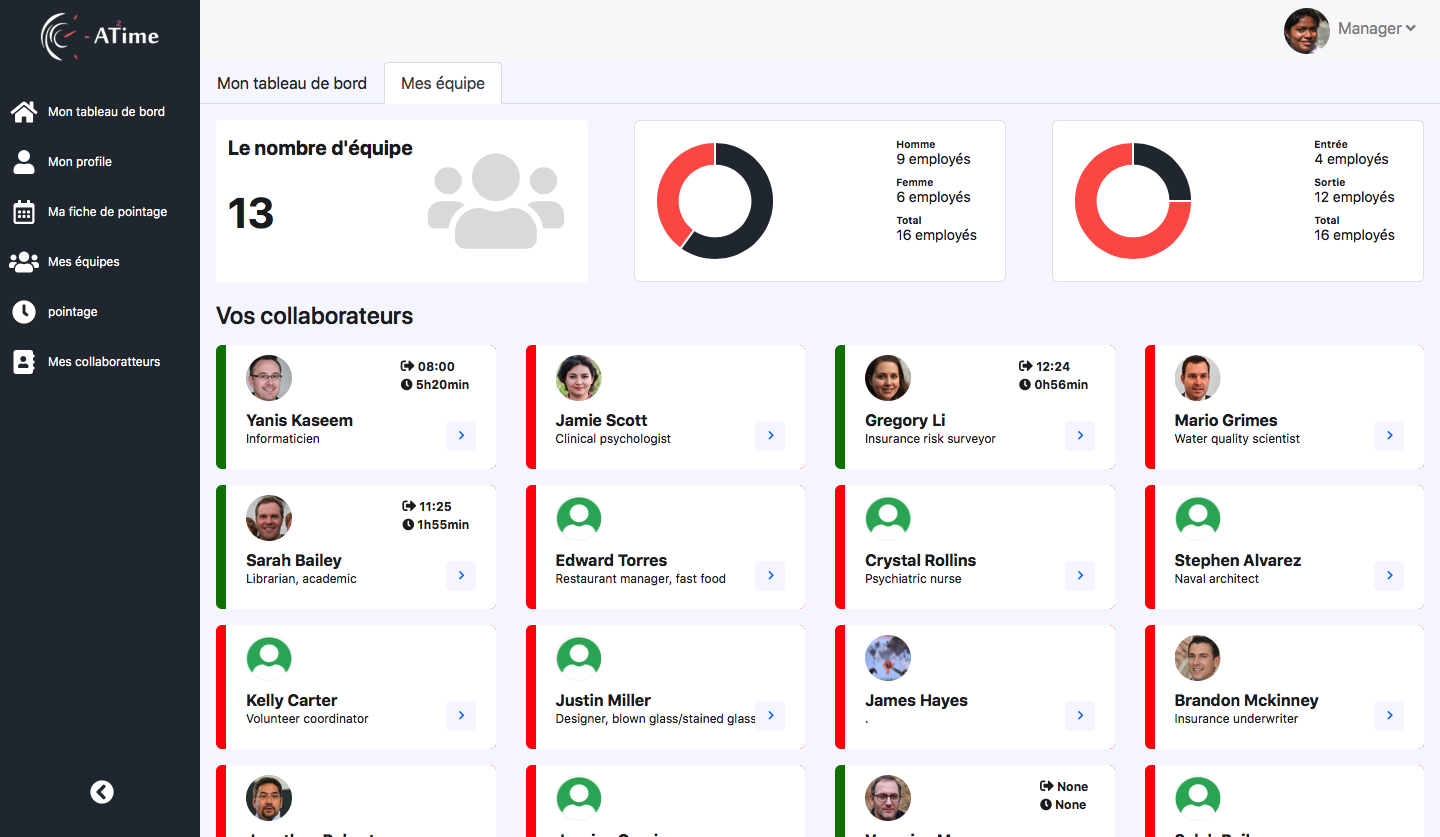
\includegraphics[scale=0.326 ]{images/interface/dashbord_manager.png}
    \caption{Interface dashbord manager}
    \label{fig96}
\end{figure}

\subsubsection*{Interface résumer d'une équipe}
Après avoir sélectionné une équipe, le manager est redirigé vers l'interface 
ci-dessous qui lui permet d'avoir une vue d'ensemble, afin de superviser les 
membres de cette dernière.

\begin{figure}[h!]
    \centering
    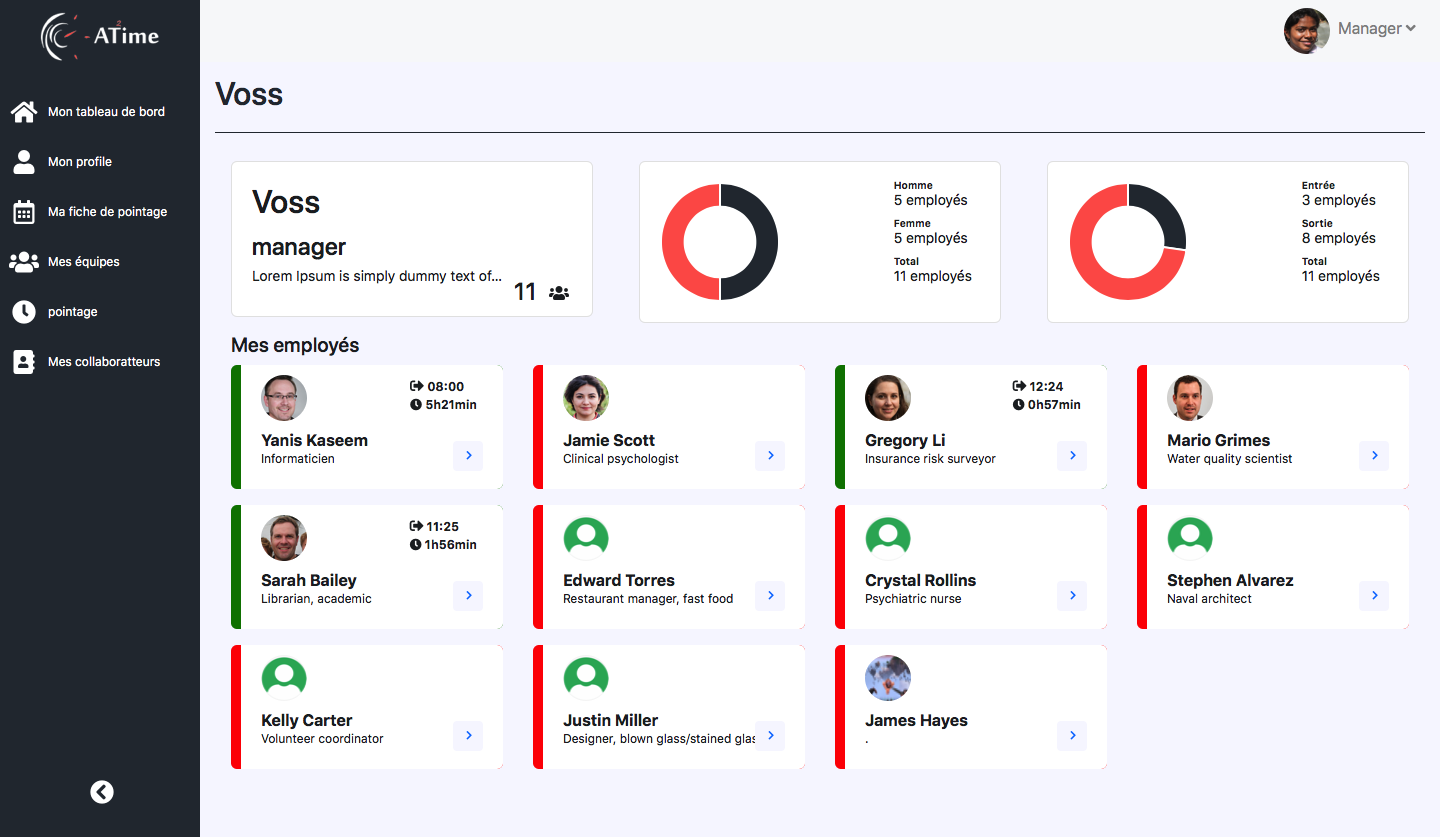
\includegraphics[scale=0.35 ]{images/interface/team_view.png}
    \caption{Interface résumer d'une équipe}
    \label{fig97}
\end{figure}

\subsection{Espace responsable}
Cet espace offre au responsable des fonctionnalités avancées avec un accès à la
totalité des informations lui permettant de contrôler et d’analyser la situation
dans laquelle se trouve l’entreprise, et ce afin de prendre des décisions en vue
d’atteindre un ou plusieurs objectifs.

\clearpage
\begin{figure}[h!]
    \centering
    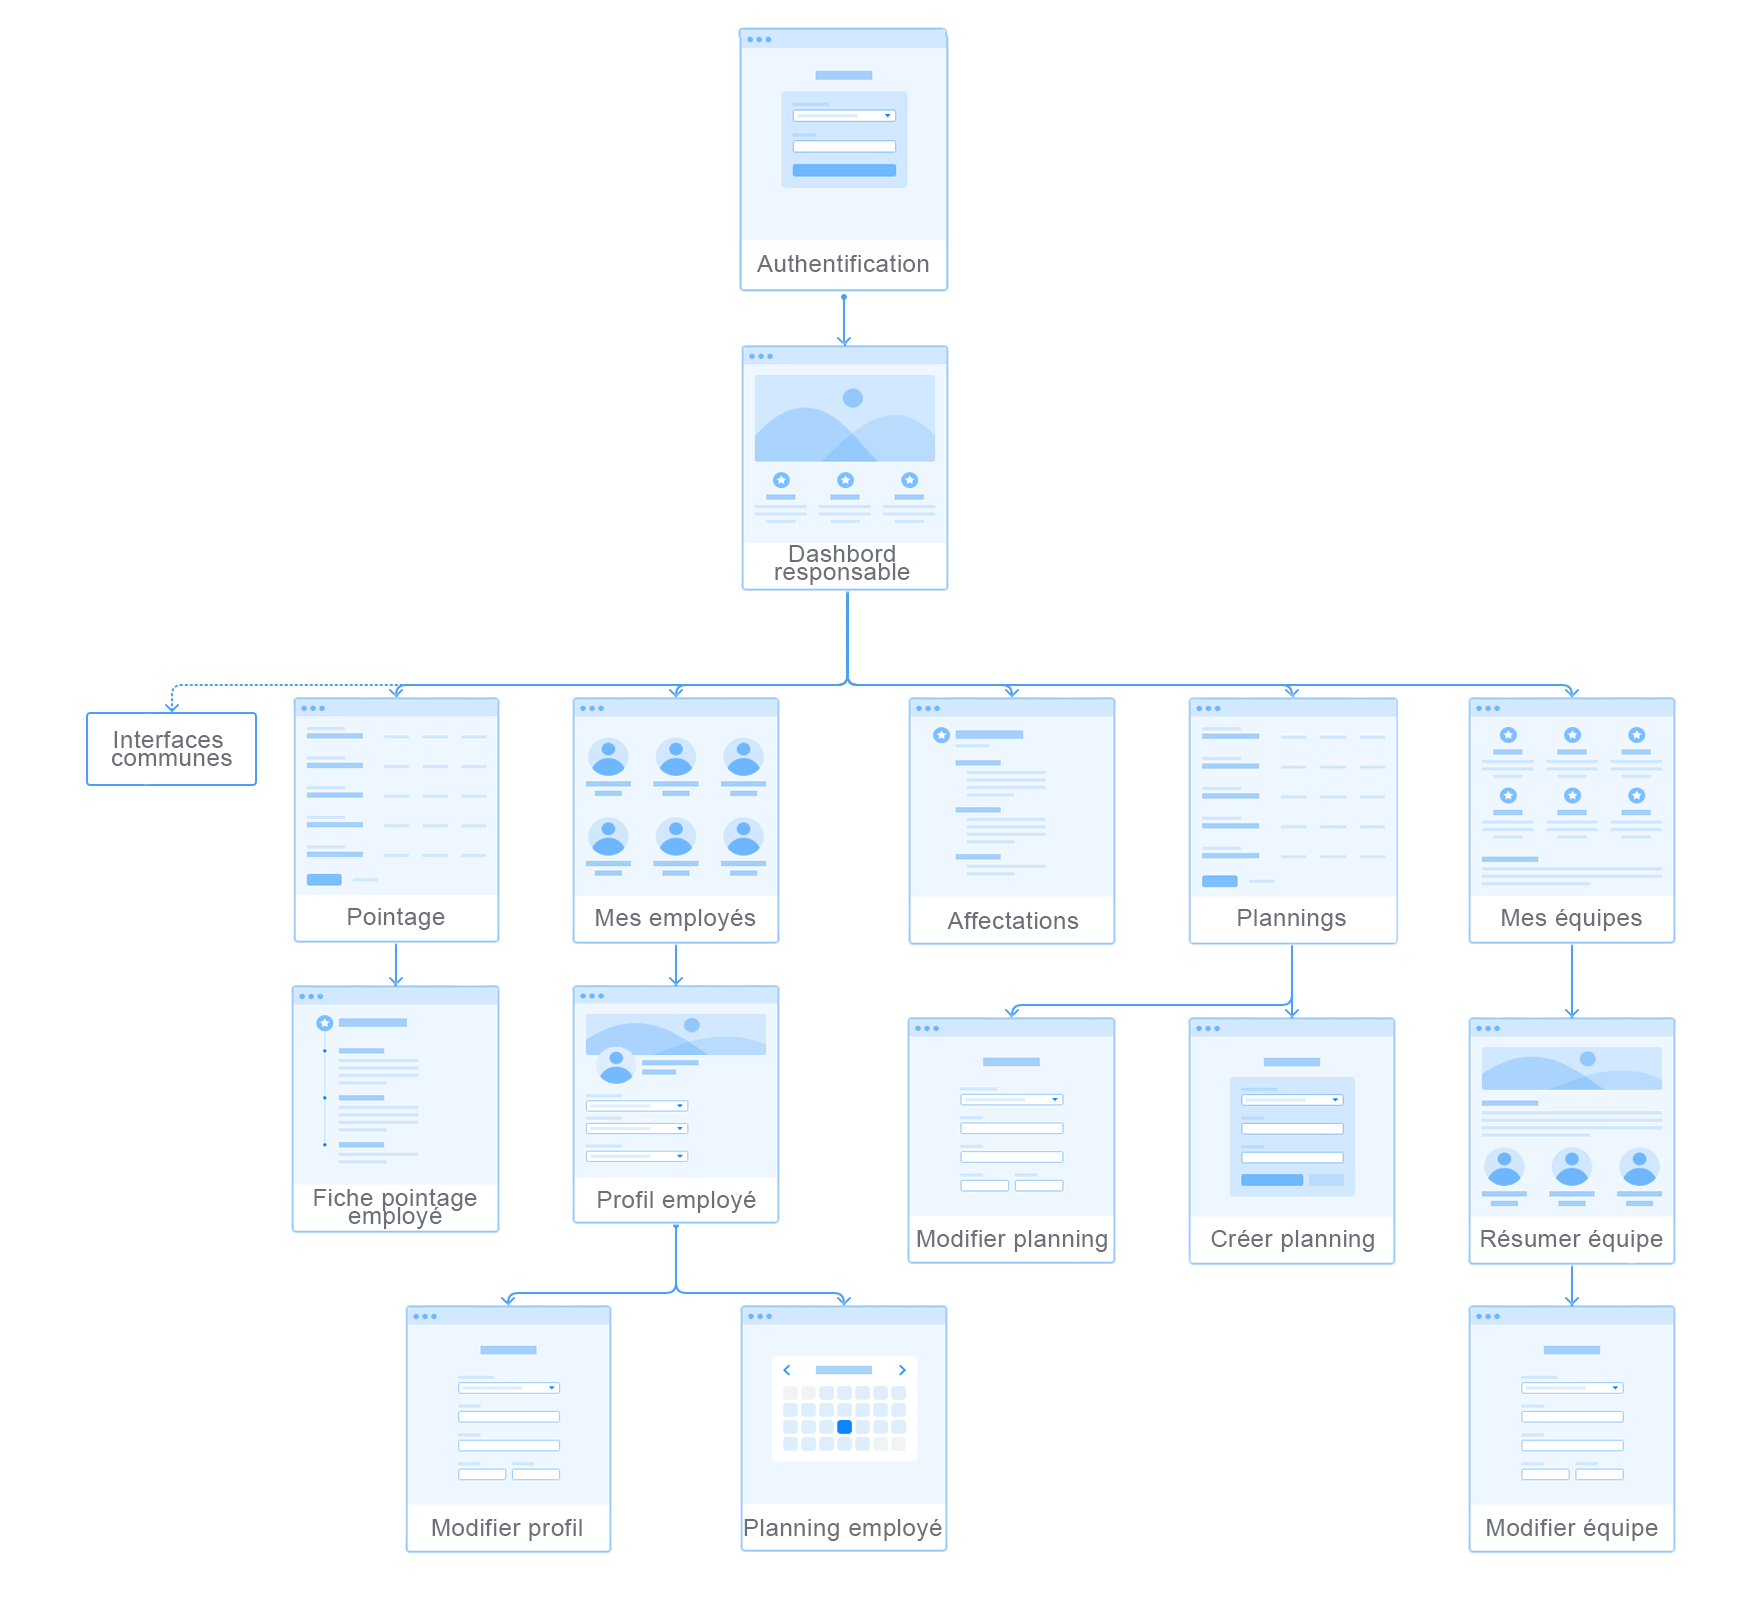
\includegraphics[scale=0.3]{images/interface/Espace responsable.png}
    \caption{User flow du responsable}
    \label{fig98}
\end{figure}

\subsubsection*{Interface créer planning}
La figure \ref{fig99} présente l'interface qui permet au responsable de créer un
planning. C'est un formulaire qui comporte le nom et une description du planning
ainsi que les horaires de travail durant la semaine.

\clearpage

\begin{figure}[h!]
    \vspace{-10pt}
    \centering
    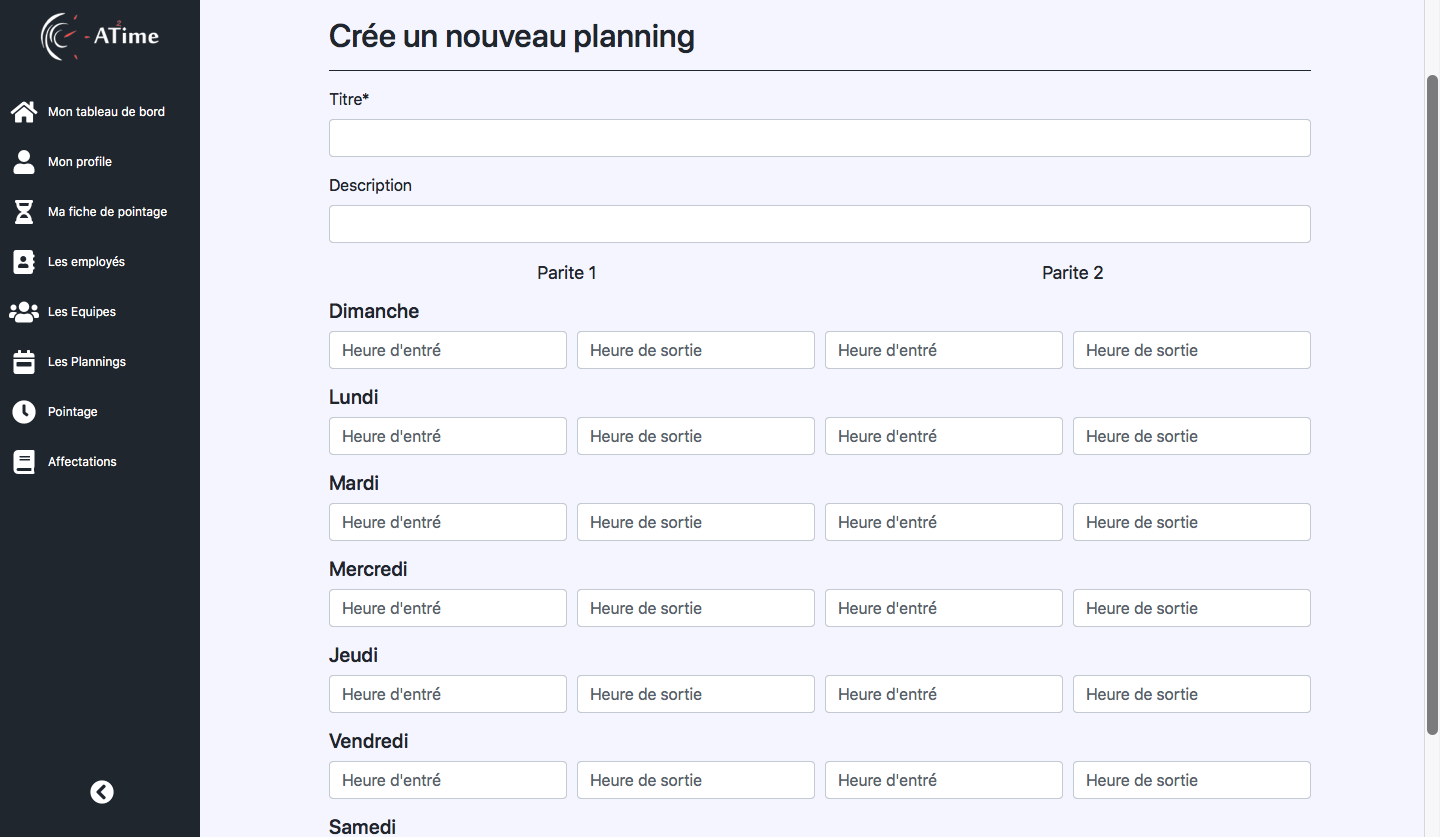
\includegraphics[scale=0.305 ]{images/interface/add_planning.png}
    \caption{interface créer un planning}
    \label{fig99}
\end{figure}

\vspace{-20pt}
\subsubsection*{Interface affecter un employé}
Une fois que le responsable sélectionne une équipe, il sera redirigé vers
l'interface qui est présentée dans la figure \ref{fig100}, elle lui permet de
consulter les informations de l'équipe ainsi que d'affecter un employé à cette
dernière en effectuant une recherche avec son nom et prénom dans le champ
correspondant. 

\begin{figure}[h!]
    \centering
    \includegraphics[scale=0.305 ]{images/interface/résumer_team.png}
    \caption{Interface affecter un employé}
    \label{fig100}
\end{figure}

\clearpage

\subsection{Espace administrateur}
Cet espace permet à l’administrateur d’avoir accès de manière structurée à la 
base de données. Ainsi, il peut assurer la cohérence des données de l’entreprise 
grâce aux quatre fonctions de base CRUD lui permettant de créer, lire, mettre à 
jour, et supprimer des données.

\subsection*{Interface Ajouter employé}
Une fois authentifié, l’administrateur pourra à travers cette interface qui se
présente sous la forme d’un formulaire d'ajout d'un employé. Il doit renseigner
les informations les plus sensibles pour le bon fonctionnement du système.  

\begin{figure}[h!]
    \centering
    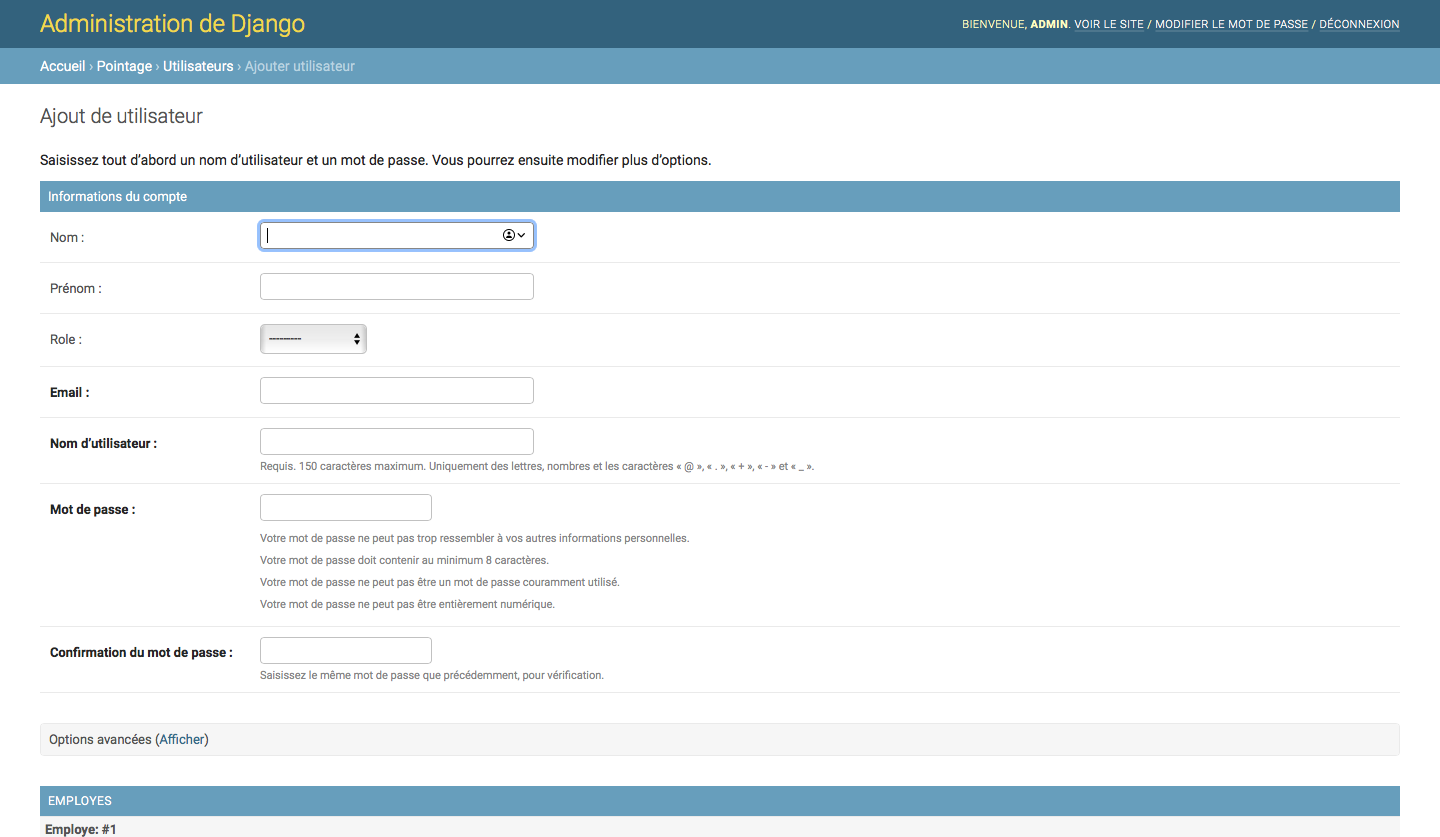
\includegraphics[scale=0.35]{images/interface/admin_add_employe.png}
    \vspace{-20pt}
    \caption{User flow de l'administrateur}
    \label{fig101}
\end{figure}

\section{Sécurité de l’application}
La sécurité des applications Web est devenue un enjeu stratégique aussi
important que les fonctionnalités ou l’ergonomie. Pour cela, Django nous a
permis de mettre en place des mesures de sécurité contre plusieurs types
d’attaques.

\subsection{Protection contre Cross Site Scripting}
Le Cross-Site-Scripting, ou XSS, est la technique d'exploitation des 
applications Web pour inciter les navigateurs des utilisateurs à exécuter du 
JavaScript malveillant pour par exemple:

\begin{itemize}
    \item[\textbullet] Changer les mots de passe des utilisateurs à leur insu.
    \item[\textbullet] Collecter de données.
    \item[\textbullet] Exécuter des actions arbitraires.
\end{itemize}

Django suppose que toutes les données de contexte sont non sécurisées, sauf sur 
indication contraire. Cela signifie que la plupart des formes d'attaque XSS ne 
fonctionnent pas avec les modèles Django.

\subsection{Protection contre Cross site request forgery}
Les attaques CSRF permettent à un utilisateur malveillant d'exécuter des actions 
en utilisant les informations d'identification d'un autre utilisateur à son insu 
ou sans son consentement.

Le middleware CSRF et le template tag csrf token de Django permet une protection 
facile à mettre en place contre la plupart des types d'attaques CSRF.

\subsection{Protection contre SQL injection}
L'injection SQL est un type d'attaque où un utilisateur malveillant est capable 
d'exécuter du code SQL arbitraire sur une base de données. Cela peut entraîner 
la suppression d'enregistrements ou une fuite de données.

L’ORM de Django est une protection contre ce type d’attaque, il permet de 
protéger les requêtes en les construisant à l'aide du paramétrage des requêtes.

\subsection{Protection contre le Clickjacking}
Le détournement de clic est un type d'attaque où un site malveillant enveloppe 
un autre site. Ce type d’attaques se produit lorsqu’un site malveillant piège un 
utilisateur pour qu’il clique sur un élément caché d’un autre site que le site 
malveillant a chargé. 

Les middlewares et décorateurs de Django fournissent une protection facile à 
utiliser contre le détournement de cliques.

\section{Tests}
La phase de test est une partie fondamentale du processus de développement 
d’application. Afin de nous assurer de la qualité et fiabilité de notre 
application, nous avons effectué des tests tout au long du développement ce qui 
nous a permis d’avoir une détection précoce des erreurs et de les corriger dès 
que possible.

\section{Conclusion}
Dans ce chapitre nous avons énoncé les différents logiciels, plateformes,
libraires utilisés pour la réalisation de notre application. À savoir le
framework Django, et le langage de programmation Python et ses différents
packages.  Suite à cela, nous avons présenté notre application sous différentes
facettes que ce soit le côté persistance de données, la charte graphique, la
hiérarchie des pages, les interfaces, et la sécurité.
